\documentclass{article}
\usepackage{tikz, hyperref, comment, amsmath, cleveref, forest, subcaption, listings, xcolor, float}
\usepackage[bottom]{footmisc}
\usepackage[margin=.75in]{geometry}

\renewcommand{\contentsname}{Indice}
\renewcommand{\refname}{Riferimenti}
\renewcommand{\figurename}{Figura}
\renewcommand{\tablename}{Tabella}
\renewcommand{\lstlistingname}{Listato}

\crefformat{section}{\S#2#1#3}
\crefformat{subsection}{\S#2#1#3}
\crefformat{subsubsection}{\S#2#1#3}
\crefformat{figure}{#2Figura~#1#3}
\crefformat{footnote}{#2\footnotemark[#1]#3}
\crefformat{table}{#2Tabella~#1#3}

\crefname{lstlisting}{listato}{listati}
\Crefname{lstlisting}{Listato}{Listati}

\usepackage[listings,skins]{tcolorbox}
\lstdefinelanguage{Toml}{
    comment = [l]{\#},
    keywords = {true, false},
    morestring = [b]{"}
}

\lstset{
    tabsize = 2,
    frame = tb,
    breaklines = true,
    numbers = left,
    numbersep = 5pt,
    numberstyle = \color{white!30!black}\scriptsize,
    stepnumber = 1,
    basicstyle = \footnotesize\ttfamily,
    commentstyle={\color{green!50!black}\ttfamily},
    keywordstyle = {\bfseries\color{purple}}, % keywords
    keywordstyle = [2]{\itshape\color{blue}}, % traits
    keywordstyle = [3]{\color{blue}}, % primitive types
    keywordstyle = [4]{\color{blue}}, % type and value ctors
    keywordstyle = [5]{\color{purple!50!blue}}, % macros
    stringstyle = \color{green!45!blue},
    aboveskip = \baselineskip,
    showstringspaces = false
}
 \lstdefinelanguage{docker}{
  keywords={FROM, RUN, COPY, ADD, ENTRYPOINT, CMD,  ENV, ARG, WORKDIR, EXPOSE, LABEL, USER, VOLUME, STOPSIGNAL, ONBUILD, MAINTAINER, HEALTHCHECK},
  keywordstyle=\color{blue}\bfseries,
  identifierstyle=\color{black},
  sensitive=false,
  comment=[l]{\#},
  commentstyle=\color{purple}\ttfamily,
  stringstyle=\color{red}\ttfamily,
  morestring=[b]',
  morestring=[b]"
}

\title{High performance and quantum computing}

\author{Giuseppe Capasso}

\begin{document}
\begin{titlepage}
  \thispagestyle{empty}
  \raggedright % Allinea a sinistra

  \begin{tikzpicture}
    \node[anchor=south west] at (4,0) {
\includegraphics[scale=0.75]{figures/unina-logo-1.png}};
    \node[anchor=south west] at (0,1.5) {
\includegraphics{figures/unina-logo-2.png}};
    \node[anchor=south west] at (0,0.5) {\textsf{Scuola Politecnica e delle Scienze di Base}};
    \node[anchor=south west] at (0,0) {\textsf{Corso di Laurea Magistrale in Ingegneria Informatica}};
  \end{tikzpicture}

  \vfill

  {\textbf{\textit{\LARGE Tracing e profiling di applicazioni SGX in Linux}}}
  \\[2cm]

  {\textbf{\textit{\Large High Performance and Quantum Computing}}}
  \\[1cm]
  {\large Anno Accademico 2024/2025}

  \vfill

  \begin{table}[h]
    \textbf{Giuseppe Capasso matr. M63001498}
  \end{table}

\end{titlepage}

\thispagestyle{empty}
\tableofcontents

\newpage
\thispagestyle{empty}

\section*{Introduzione}
L'implementazione di Trusted Execution Environment (TEE) in hardware contrasta alcuni \textit{threat model} a discapito delle performance delle applicazioni. Lo scopo di questo progetto è quello di creare un sistema che consenta di raccogliere metriche di applicazioni sia quando vengono eseguite in TEE che non per effettuarne delle comparazioni in futuro. La difficoltà principale nella raccolta metriche in questo tipo di scenari è l'uniformità. Infatti, in TEE hardware, il sistema operativo è visto come non fidato e quindi viene utilizzato in meno possibile dalle applicazioni che potrebbero disabilitare per motivi di sicurezza la raccolta metriche.
L'implementazione proposta si basa su Intel-SGX e utilizza Gramine. Gramine è uno strumento proposto da Intel per effettuare il porting di applicazioni già esistenti in TEE evitando di modificare il codice sorgente.

\clearpage
\section{Requisiti}\label{sec:requirements}
Il sistema che si vuole costruire deve essere in grado di orchestrare l'esecuzione di benchmark di più programmi, eseguendo ogni programma sia con Gramine che senza, variando diverse metriche. I requisiti dell'applicazione sono riassunti nella seguente tabella:

\begin{table}[h]
\centering
\begin{tabular}{|l|p{10cm}|}
\hline
\textbf{Requisito} & \textbf{Descrizione} \\ \hline
R1 & L'applicazione deve essere in grado di eseguire programmi in un ambiente Trusted Execution Environment (TEE) utilizzando Gramine. \\ \hline
R2 & L'applicazione deve eseguire gli stessi programmi anche al di fuori del TEE per consentire il confronto delle prestazioni. \\ \hline
R3 & Deve essere possibile variare le metriche di esecuzione, come il numero di thread, la quantità di memoria allocata, e altre risorse di sistema. \\ \hline
R4 & L'applicazione deve raccogliere metriche di performance durante l'esecuzione dei programmi, sia in TEE che non. \\ \hline
R5 & Deve essere garantita l'uniformità nella raccolta delle metriche, indipendentemente dall'ambiente di esecuzione. \\ \hline
R6 & L'applicazione deve fornire un'interfaccia per configurare e avviare i benchmark in modo automatizzato. \\ \hline
R7 & I risultati dei benchmark devono essere salvati in un formato che consenta un'analisi successiva. \\ \hline
R8 & L'applicazione deve essere in grado di gestire errori e anomalie durante l'esecuzione dei benchmark, fornendo log dettagliati. \\ \hline
R9 & Deve essere possibile eseguire benchmark su diverse piattaforme hardware supportate da Intel-SGX. \\ \hline
\end{tabular}
\caption{Requisiti dell'applicazione per il benchmarking in TEE e non-TEE}
\end{table}

Il benchmark si divide in due tipi principali: Macro benchmark e Micro benchmark. In questa sezione ci concentreremo sui parametri del Macro benchmark, che riguardano l'esecuzione in enclave. I parametri considerati sono i seguenti:

\begin{table}[h]
\centering
\begin{tabular}{|l|p{6cm}|p{6cm}|}
\hline
\textbf{Parametro} & \textbf{Descrizione} & \textbf{Note} \\ \hline
Enclave & Indica se l'esecuzione avviene all'interno di un enclave (Sì/No). & \\ \hline
Memoria Enclave & La quantità di memoria dedicata all'enclave, con valori come "256M". &  A seconda della versione di SGX considerata questo comporterà l'allocazione statica (SGX1) o dinamica (SGX2) della memoria. La memoria EPC ha una grandezza standard che viene configurata dal BIOS e può essere di 64M o 128M  \\ \hline
Numero di thread & Il numero di thread utilizzati dal programma durante l'esecuzione. & A seconda della versione di SGX il numero di thread può crescere staticamente o dinamicamente. Per SGX1, un'enclave ha bisogno di almeno $4$ thread per eseguire (gestore Gramine, servizi di attestazione remota etc.); mentre SGX2 può creare dinamicamente i thread quando c'è bisogno \\ \hline
Tipo di storage & Specifica se lo storage è non fidato (untrusted) o cifrato (encrypted). & \\ \hline
\end{tabular}
\caption{Parametri del Macro benchmark}
\end{table}

Questi parametri sono fondamentali per valutare le prestazioni delle applicazioni quando vengono eseguite in un ambiente Trusted Execution Environment (TEE) utilizzando Gramine. La configurazione di questi parametri consente di analizzare l'impatto delle diverse risorse e configurazioni sull'efficienza e la sicurezza delle applicazioni.

I parametri del micro benchmark sono fondamentali per analizzare il comportamento dettagliato delle applicazioni. I parametri considerati sono i seguenti:

\begin{table}[h]
\centering
\begin{tabular}{|l|p{6cm}|p{6cm}|}
\hline
\textbf{Parametro} & \textbf{Descrizione} & \textbf{Note} \\ \hline
Consumo energetico & Misura l'energia consumata durante l'esecuzione di applicazioni Gramine e non &  \\ \hline
Tracce di esecuzione & Raccoglie le tracce di esecuzione per analizzare il flusso del programma. &  \\ \hline
Pattern di accesso & Analizza i pattern di accesso alla memoria e alle risorse. &  \\ \hline
\end{tabular}
\caption{Parametri del Micro benchmark}
\end{table}

\clearpage
\section{Strumenti per il profiling in Linux}

In questo capitolo si analizzano i principali strumenti messi a disposizione da Linux per il monitoraggio e l'analisi delle prestazioni dei sistemi. In particolare, verranno esaminati i meccanismi basati sui performance counters, le tecniche di misurazione dell'energia e il tracing a livello kernel tramite eBPF.

\subsection{Performance counters}

I performance counters sono strumenti hardware che consentono di monitorare eventi interni alla CPU, come il numero di cicli, cache misses e altri eventi critici per l'analisi delle prestazioni. Linux fornisce l'interfaccia \texttt{perf}, utilizzabile sia come utility da linea di comando sia in maniera programmatica tramite la system call \texttt{perf\_event\_open}.

La system call \texttt{perf\_event\_open} apre un descrittore di file che rappresenta un contatore di performance. La struttura \texttt{perf\_event\_attr} viene utilizzata per specificare il tipo di evento da monitorare (ad es. cicli CPU, eventi hardware, ecc.), le modalità di raccolta e altre opzioni, come l'esclusione delle attività in kernel o in ambienti virtualizzati.

Di seguito è riportato uno snippet di codice in C che illustra un esempio basilare di utilizzo di \texttt{perf\_event\_open} per monitorare il numero di cicli della CPU:

\begin{lstlisting}[language=C, caption={Esempio di utilizzo di \texttt{perf\_event\_open} per contare i cicli CPU}]
#include <stdio.h>
#include <stdlib.h>
#include <string.h>
#include <unistd.h>
#include <linux/perf_event.h>
#include <sys/ioctl.h>
#include <sys/syscall.h>
#include <asm/unistd.h>
#include <errno.h>

/* Funzione wrapper per la system call perf_event_open */
static long
perf_event_open(struct perf_event_attr *hw_event, pid_t pid, int cpu,
                int group_fd, unsigned long flags) {
    return syscall(__NR_perf_event_open, hw_event, pid, cpu, group_fd, flags);
}

int main(void) {
    struct perf_event_attr pe;
    long fd;
    long long count;

    /* Inizializza la struttura a zero e configura l'evento da monitorare */
    memset(&pe, 0, sizeof(struct perf_event_attr));
    pe.type = PERF_TYPE_HARDWARE;
    pe.size = sizeof(struct perf_event_attr);
    pe.config = PERF_COUNT_HW_CPU_CYCLES;
    pe.disabled = 1;
    pe.exclude_kernel = 1;
    pe.exclude_hv = 1;

    /* Apre il contatore per il processo corrente su tutti i core (-1) */
    fd = perf_event_open(&pe, 0, -1, -1, 0);
    if (fd == -1) {
        perror("perf_event_open");
        exit(EXIT_FAILURE);
    }

    ioctl(fd, PERF_EVENT_IOC_RESET, 0);
    ioctl(fd, PERF_EVENT_IOC_ENABLE, 0);

    /* Inserire qui il lavoro da monitorare */
    sleep(1);

    ioctl(fd, PERF_EVENT_IOC_DISABLE, 0);
    read(fd, &count, sizeof(long long));
    printf("CPU cycles: %lld\n", count);

    close(fd);
    return 0;
}
\end{lstlisting}

In questo esempio, la struttura \texttt{perf\_event\_attr} viene configurata per contare i cicli CPU (\texttt{PERF\_COUNT\_HW\_CPU\_CYCLES}) escludendo il codice kernel e le operazioni in ambienti virtualizzati. Dopo aver aperto il contatore tramite \texttt{perf\_event\_open}, il contatore viene resettato, abilitato, e successivamente disabilitato per leggere il valore accumulato, che viene stampato a video.

\subsection{Misurazione dell'energia}
La tecnologia \emph{Running Average Power Limit (RAPL)} consente di monitorare il consumo energetico del sistema suddividendolo in in domini di potenza, quali \textit{package}, \textit{core}, \textit{uncore} e \textit{DRAM},  sfruttando contatori hardware che vengono incrementati in base alla corrente e alla tensione misurate. Questi contatori forniscono una stima dell'energia consumata, espressa in microjoule, e sono esposti dal kernel Linux tramite il filesystem \texttt{sysfs}.

\paragraph{Interfaccia Sysfs}

L'interfaccia RAPL è accessibile in Linux all'interno della directory:

\begin{forest}
for tree={
    font=\ttfamily,
    grow'=0,
    child anchor=west,
    parent anchor=south,
    anchor=west,
    calign=first,
    edge path={
      \noexpand\path [draw, \forestoption{edge}]
      (!u.south west) +(7.5pt,0) |- node[fill,inner sep=1.25pt] {} (.child anchor)\forestoption{edge label};
    },
    before typesetting nodes={
      if n=1
        {insert before={[,phantom]}}
        {}
    },
    fit=band,
    before computing xy={l=15pt},
  }
  [/sys/devices/virtual/powercap
          [intel-rapl
            [enabled]
            [intel-rapl:i
              [enabled]
              [energy\_uj]
              [max\_energy\_range\_uj]
              [name]
              [intel-rapl:i:j
                [enabled]
                [energy\_uj]
                [max\_energy\_range\_uj]
                [name]
              ]
            ]
          ]
        ]
      ]
    ]
  ]
\end{forest}

In questa struttura, l'indice \texttt{i} rappresenta il dominio energetico principale (ad esempio, un package CPU) e l'indice \texttt{j} identifica eventuali sotto-domini (ad esempio, i core interni o la DRAM). Il file \texttt{energy\_uj} contiene il valore cumulativo dell'energia consumata in microjoule, mentre \texttt{max\_energy\_range\_uj} specifica il massimo valore raggiungibile prima che il contatore si resetti.

\paragraph{Implementazione e limiti di RAPL}

I contatori RAPL sono implementati direttamente in hardware:  
\begin{itemize}
    \item \textbf{Misurazione hardware:} Il consumo energetico viene stimato in base alla corrente e alla tensione rilevate da sensori integrati, aggiornando continuamente i contatori.
    \item \textbf{Modelli interni:} I valori riportati sono basati su modelli interni del processore, il che può comportare una certa discrepanza rispetto al consumo reale, soprattutto in condizioni di carico variabile.
    \item \textbf{Risoluzione e wrap-around:} La risoluzione tipica in microjoule potrebbe non essere sufficiente per analisi ad altissima frequenza, e, essendo contatori cumulativi, se non letti con sufficiente frequenza, possono raggiungere il loro limite massimo e conseguentemente "wrap-around", rendendo necessaria una gestione attenta per evitare errori di interpretazione.
\end{itemize}

\subsubsection{Consumo energetico di un disco}
Lo standard RAPL è stato proposto da Intel e implementato anche su alcuni processori AMD. Tuttavia, non esiste uno standard per misurare il consumo energetico di un disco, ma possono essere ottenute delle metriche indirette a partire dal numero di byte scritti, conoscendo la configurazione di base del sistema e le specifiche del disco utilizzate.

Ad esempio, assumendo di avere un disco rotazionale con 7200rpm, il consumo energetico può variare in base al tipo di operazione di scrittura. Supponiamo che il consumo medio per una scrittura sequenziale di 1GB sia di circa 5W, mentre per una scrittura casuale sia di circa 10W, a causa del maggiore movimento delle testine. Se ipotizziamo di scrivere un totale di \(x\) byte, di cui il 70\% in modalità sequenziale e il 30\% in modalità casuale, il consumo energetico totale può essere stimato come segue:

\begin{itemize}
  \item Consumo per scrittura sequenziale: \(0.7 \times \frac{x}{1 \text{GB}} \times 5 \text{W}\);
  \item Consumo per scrittura casuale: \(0.3 \times \frac{x}{1 \text{GB}} \times 10 \text{W}\)
\end{itemize}

I dischi SSD (e nvme) non risentono della differenza di operazioni sequenziali e randomiche.

\subsection{Tracing a livello kernel: eBPF}
\emph{extended Berkeley Packet Filter (eBPF)} è una tecnologia utilizzata per eseguire programmi all'interno del kernel senza scrivere un modulo. Il vantaggio di questa scelta risiede nel fatto che l'ambiente in cui eseguono questi programmi è isolato e, pertanto, un \textit{crash} del programma non impatta il fallimento del kernel.

Un programma eBPF è composto da diverse sezioni, tra cui le sezioni `.maps`, che definiscono le strutture dati utilizzate per memorizzare le informazioni raccolte durante l'esecuzione. Queste mappe sono essenziali per trasferire i dati dal kernel allo spazio utente. Un aspetto distintivo dei programmi eBPF è che non hanno un punto di ingresso `main` come i programmi tradizionali. Invece, vengono attaccati (attraverso la primitiva \textbf{\textit{attach}}) a specifici eventi o punti di hook nel kernel, come l'entrata o l'uscita da una system call.

\subsubsection{Architettura eBPF}
eBPF è una macchina virtuale (simile alla JVM) instanziata all'interno del kernelper l'esecuzione di programmi. La macchina è di tipo RISC e ha $11$ registri a $64-bit$, uno stack limitato a $512$ byte. Questa macchina effettua dei salti alle istruzioni da eseguire utilizzando una coda dei programmi.

Questa macchina è dotata di un JIT (Just in time compiler) che consente di compilare in codice macchina il codice oggetto passato in ingresso, generate con un compilatore \textit{LLVM-compliant}. Come mostrato in \cref{fig:ebpf_arch}, prima di essere caricato in memoria, il programma passa per un \textit{verifier}. Questo applica delle regole per capire se:
\begin{itemize}
  \item il programma effettua cicli infiniti;
  \item accede ad aree di memoria illecite e/o non inizializzate
\end{itemize}

\begin{figure}
  \begin{center}
    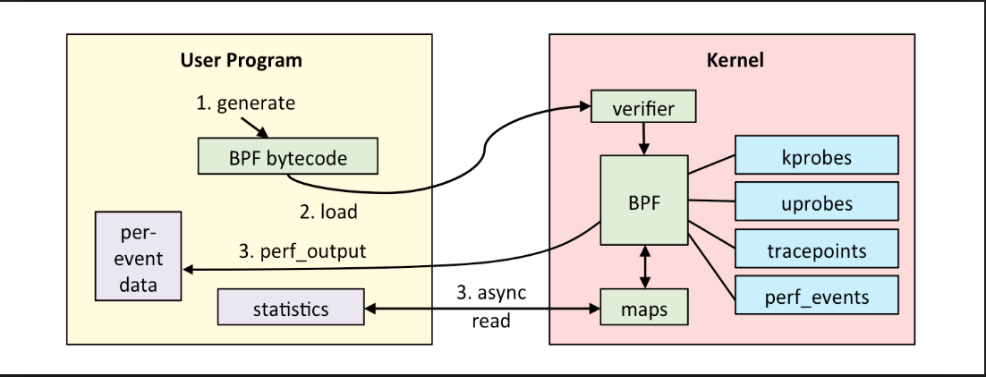
\includegraphics[width=0.95\textwidth]{./figures/ch2/ebpf_arch.png}
  \end{center}
  \caption{Flusso di un programma eBPF}\label{fig:ebpf_arch}
\end{figure}


\paragraph{Struttura di un programma eBPF} Di seguito è riportato un programma eBPF che invia in spazio utente ogni volta che viene chiamata la system call \texttt{read}. Il programma dichiara un ringbuffer a cui si dovrà sottoscrivere il programma user-space per ottenere gli eventi.
\begin{lstlisting}[language=C, caption={Esempio di un programma eBPF che invia in user-space tutte le operazioni sys\_enter\_read}]
#include <linux/bpf.h>
#include <bpf/bpf_helpers.h>

#define EVENT_SYS_READ 0

struct event {
  __u32 ev_type;
  __u64 timestamp;
};

struct {
  __uint(type, BPF_MAP_TYPE_RINGBUF);
  __uint(max_entries, 1 << 20);
} events SEC(".maps");

static __always_inline int snd_trace_event(__u32 evt) {
  __u64 ts = bpf_ktime_get_ns();
  struct event *rb_event = bpf_ringbuf_reserve(&events, sizeof(struct event), 0);

  if (!rb_event) {
    bpf_printk("bpf_ringbuf_reserve failed\n");
    return 1;
  }

  rb_event->ev_type = evt;
  rb_event->timestamp = ts;

  bpf_ringbuf_submit(rb_event, 0);

  return 0;
}

SEC("tracepoint/syscalls/sys_enter_read")
int trace_enter_read(struct trace_event_raw_sys_enter *ctx) {
  return snd_trace_event(EVENT_SYS_READ); 
}

char LICENSE[] SEC("license") = "GPL";
\end{lstlisting}

Questo programma può essere compilato con:
\begin{verbatim}
clang -O2 -target bpf -g -c <file> -o <output-file>
\end{verbatim}

Utilizzando \textit{bpftool}, è possibile osservare il seguente disassemblato:
\begin{verbatim}
0: R1=ctx() R10=fp0
; __u64 ts = bpf_ktime_get_ns(); @ test.bpf.c:15
0: (85) call bpf_ktime_get_ns#5       ; R0_w=scalar()
1: (bf) r7 = r0                       ; R0_w=scalar(id=1) R7_w=scalar(id=1)
2: (b7) r6 = 0                        ; R6_w=0
; bpf_ringbuf_reserve(&events, sizeof(struct event), 0); @ test.bpf.c:17
3: (18) r1 = 0xffff9ab6d0e11700       ; R1_w=map_ptr(map=events,ks=0,vs=0)
5: (b7) r2 = 16                       ; R2_w=16
6: (b7) r3 = 0                        ; R3_w=0
7: (85) call bpf_ringbuf_reserve#131          ; R0=ringbuf_mem_or_null(id=3,ref_obj_id=3,sz=16) refs=3
; if (!rb_event) { @ test.bpf.c:19
8: (55) if r0 != 0x0 goto pc+6        ; R0=0
; bpf_printk("bpf_ringbuf_reserve failed\n"); @ test.bpf.c:20
9: (18) r1 = 0xffff9ab684678108       ; R1_w=map_value(map=test.rodata,ks=4,vs=28)
11: (b7) r2 = 28                      ; R2_w=28
12: (85) call bpf_trace_printk#6
\end{verbatim}

Il programma di seguito carica quello ebpf e stampa tutti gli eventi ricevuti dal ringbuffer.

\begin{lstlisting}[language=C, caption={Esempio di un programma user-space che riceve gli eventi dal ringbuffer}]
#include <stdio.h>
#include <stdlib.h>
#include <signal.h>
#include <bpf/libbpf.h>
#include <bpf/bpf.h>
#include "ebpf_prog.skel.h" // Autogenerato con bpftool o libbpf

static volatile int stop;

struct event {
    __u32 ev_type;
    __u64 timestamp;
};

// Gestione del segnale per terminare il programma in modo pulito
void handle_signal(int signo) {
    stop = 1;
}

// Callback per processare i dati dalla ring buffer
void handle_event(void *ctx, void *data, size_t data_sz) {
    struct event *e = (struct event *)data;
    printf("Evento ricevuto: tipo=%u, timestamp=%llu ns\n", e->ev_type, e->timestamp);
}

int main() {
    struct ring_buffer *rb = NULL;
    struct ebpf_prog *skel;
    int err;

    // Carica e attacca il programma eBPF
    skel = ebpf_prog__open_and_load();
    if (!skel) {
        fprintf(stderr, "Errore nel caricamento del programma eBPF\n");
        return 1;
    }

    err = ebpf_prog__attach(skel);
    if (err) {
        fprintf(stderr, "Errore nell'aggancio del programma eBPF: %d\n", err);
        goto cleanup;
    }

    signal(SIGINT, handle_signal);
    signal(SIGTERM, handle_signal);

    // Apri la ring buffer per ricevere eventi
    rb = ring_buffer__new(bpf_map__fd(skel->maps.events), handle_event, NULL, NULL);
    if (!rb) {
        fprintf(stderr, "Errore nell'apertura della ring buffer\n");
        goto cleanup;
    }

    printf("In ascolto degli eventi... (Ctrl+C per terminare)\n");

    while (!stop) {
        err = ring_buffer__poll(rb, 100); // Poll con timeout di 100ms
        if (err < 0) {
            fprintf(stderr, "Errore nella ring buffer poll: %d\n", err);
            break;
        }
    }

    printf("\nTerminazione...\n");

cleanup:
    ring_buffer__free(rb);
    ebpf_prog__destroy(skel);
    return 0;
}
\end{lstlisting}

\clearpage
\section{Implementazione}
Il sistema descritto in \cref{sec:requirements} è implementato in un'applicazione CLI in Rust. Il progetto si trova in \cite{eb-repo} , mentre la documentazione è disponibile in \cite{eb-docs}.
\subsection{Architettura}
L'architettura dell'applicazione è stata progettata per eseguire in maniera automatizzata una serie di esperimenti volti a misurare le prestazioni e il consumo energetico delle applicazioni target. Il sistema integra più moduli di monitoraggio, ognuno dei quali si occupa di raccogliere metriche specifiche durante l'esecuzione del programma. In particolare, l'applicazione si avvale di:
\begin{itemize}
  \item \textbf{eBPF collector}: un modulo che sfrutta eBPF per attaccare dei programmi al kernel, in modo da tracciare eventi a basso livello come le chiamate di sistema (ad esempio, \texttt{sys\_enter\_read}) e operazioni I/O. Questi dati vengono poi memorizzati in apposite strutture dati (mappe) e salvati in file CSV.
  \item \textbf{Energy monitor}: un thread dedicato che, mediante la tecnologia RAPL, esegue il polling dei contatori energetici disponibili nel kernel. Il monitoraggio viene effettuato leggendo i file relativi ai domini di potenza (ad es. \texttt{intel-rapl:0}, \texttt{intel-rapl:0:0}, ecc.) e salvando i dati con timestamp e consumo in microjoule.
  \item \textbf{Performance counters}: un processo esterno viene lanciato per sfruttare l'interfaccia \textit{perf} del kernel, consentendo la raccolta di contatori hardware e altri eventi di performance. I dati vengono raccolti in un file \texttt{perf.csv}.
  \item \textbf{Deep tracing}: se abilitato, questo modulo effettua una raccolta di tracciamenti più dettagliati, registrando eventi rilevanti relativi ad operazioni su disco, allocazioni di memoria e altri eventi critici, mediante l'utilizzo del BPF ringbuffer.
\end{itemize}

Gli esperimenti sono generati dinamicamente in base alla combinazione di parametri definiti nel file di configurazione, quali il numero di thread (\texttt{globals.num\_threads}), la dimensione dell'enclave (\texttt{globals.enclave\_size}) e, per le applicazioni basate su Gramine, il tipo di storage (\texttt{task.storage}). Ad ogni esperimento corrisponde una specifica directory contenente, oltre ai dati raccolti, il manifesto e la firma dell'enclave (per Gramine), e le directory per i file cifrati e non cifrati.

\subsubsection{Installazione}
L'installazione del sistema prevede la corretta configurazione dell'ambiente Linux, in particolare:
\begin{itemize}
  \item \textbf{Abilitazione di eBPF}: il kernel Linux deve essere compilato con il supporto a eBPF, necessario per eseguire in modo sicuro i programmi di tracciamento a basso livello. Questo richiede che siano abilitate le relative opzioni di configurazione, come illustrato nella documentazione ufficiale di eBPF.
  \item \textbf{Supporto per i contatori di performance}: è indispensabile che il kernel supporti le opzioni \texttt{CONFIG\_PERF\_EVENT}, \texttt{CONFIG\_HW\_PERF\_EVENTS} e \texttt{CONFIG\_PROFILING} per poter utilizzare l'interfaccia \textit{perf} nella raccolta dei contatori hardware.
  \item \textbf{Interfaccia RAPL}: per la misurazione del consumo energetico, il sistema deve essere in grado di accedere all'interfaccia RAPL (Running Average Power Limit) esposta in \texttt{/sys/devices/virtual/powercap/}.
  \item \textbf{Strumenti per Gramine}: per le applicazioni basate su enclave SGX, è necessario installare gli strumenti di Gramine, inclusa la libreria Python \texttt{graminelibos}. Il processo di installazione comprende la generazione del manifesto a partire da un template in formato TOML, la verifica dei file fidati e la firma dell'enclave con una chiave privata.
\end{itemize}

\subsubsection{Configurazione}
La configurazione dell'applicazione avviene tramite un file in formato TOML che consente di specificare sia i parametri globali sia i task da eseguire. Tra i parametri globali vi sono:
\begin{itemize}
  \item \texttt{sample\_size}: il numero di volte in cui ogni esperimento deve essere ripetuto.
  \item \texttt{enclave\_size}: una lista di dimensioni da assegnare all'enclave.
  \item \texttt{num\_threads}: un array che definisce il numero di thread da utilizzare per ciascun esperimento.
  \item \texttt{extra\_perf\_events}: ulteriori eventi di performance da monitorare.
  \item \texttt{debug} e \texttt{deep\_trace}: flag per abilitare o disabilitare rispettivamente il debug e il tracciamento approfondito.
\end{itemize}
I task, invece, definiscono l'eseguibile da monitorare, gli argomenti da passare (con placeholder dinamici come \texttt{\{\{ num\_threads \}\}} e \texttt{\{\{ output\_directory \}\}}) e, per le applicazioni Gramine, il tipo di storage da utilizzare (ad es. \texttt{encrypted}, \texttt{tmpfs}, \texttt{untrusted}). Un esempio di configurazione è il seguente:
\begin{verbatim}
[globals]
sample_size = 4
enclave_size = ["256M", "512M"]
output_directory = "results"
num_threads = [1, 2, 8]
extra_perf_events = ["cpu-clock"]
debug = false
deep_trace = true

[[tasks]]
executable = "/usr/bin/make"
args = ["-C", "examples/basic-c-app/", "-j", "{{ num_threads }}", "app", "output={{ output_directory }}"]
storage_type = ["encrypted", "tmpfs", "untrusted"]
\end{verbatim}

Durante la fase di configurazione, il sistema genera in modo automatico tutte le combinazioni possibili dei parametri specificati, creando una struttura di directory per ciascun esperimento. Nel caso di applicazioni basate su Gramine, vengono inoltre generati il manifesto dell'enclave e il file di firma, insieme alle directory necessarie per i file cifrati e non cifrati.

\clearpage
\pagestyle{plain}
\pagenumbering{roman}
\setcounter{page}{1}
\addcontentsline{toc}{section}{Riferimenti}
\bibliographystyle{plain}
\bibliography{refs}

\end{document}
